\emph{On note $A$ l'évènement \og Pierre joue la manche en premier \fg{} et $G$ l'évènement \og Pierre gagne la manche \fg. On a
$P(A) = P\left(\overline{A}\right) = \dfrac{1}{2}$, $P_A(G) = \dfrac{2}{3}$ et $P_{\overline{A}}(G) = \dfrac{2}{5}$.}

\begin{enumerate}
	\item La somme des probabilités issues d'un même n{\oe}ud vaut 1 :
	$P_A\left(\overline{G}\right) = 1 - \dfrac{2}{3} = \dfrac{1}{3}$ et
	$P_{\overline{A}}\left(\overline{G}\right) = 1 - \dfrac{2}{5} = \dfrac{3}{5}$.

	\begin{center}
		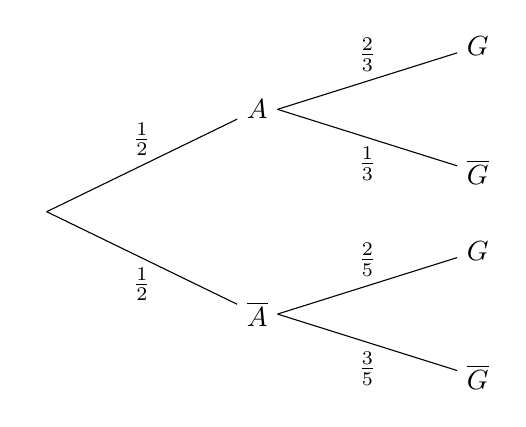
\begin{tikzpicture}[x=2.8cm, y=1cm]
			
			\node (root) at (0,0) {};
			\node (A) at (1,1.3) {$A$};
			\node (Ab) at (1,-1.3) {$\overline{A}$};
			\node (G1) at (2,2.1) {$G$};
			\node (G1b) at (2,0.5) {$\overline{G}$};
			\node (G2) at (2,-0.5) {$G$};
			\node (G2b) at (2,-2.1) {$\overline{G}$};
			
			\draw (root.east) -- (A) node[pos=0.5,above] {$\frac{1}{2}$};
			\draw (root.east) -- (Ab) node[pos=0.5,below] {$\frac{1}{2}$};
			
			\draw (A.east) -- (G1) node[pos=0.5,above] {$\frac{2}{3}$};
			\draw (A.east) -- (G1b) node[pos=0.5,below] {$\frac{1}{3}$};
			\draw (Ab.east) -- (G2) node[pos=0.5,above] {$\frac{2}{5}$};
			\draw (Ab.east) -- (G2b) node[pos=0.5,below] {$\frac{3}{5}$};
		\end{tikzpicture}
	\end{center}

	\item D'après l'énoncé : $P_A(G) = \dfrac{2}{3}$ et $P_{\overline{A}}(G) = \dfrac{2}{5}$.

	\item $P(A \cap G) = P(A) \times P_A(G) = \dfrac{1}{2} \times \dfrac{2}{3} = \dfrac{2}{6} = \dfrac{1}{3}$.

	La probabilité que Pierre joue la manche en premier et qu'il la gagne est égale à $\dfrac{1}{3}$.
\end{enumerate}
